\documentclass[border=4pt]{standalone}
% Shared typography and colours for the standalone figures.
\usepackage{unicode-math}
\setmainfont{TeX Gyre Termes}
\setmathfont{TeX Gyre Termes Math}
\usepackage{tikz}
\usetikzlibrary{arrows.meta,positioning,calc,decorations.pathreplacing}
\usepackage{pgfplots}
\pgfplotsset{compat=1.18}

% One colour per element or subsystem. Record the mapping in
% the working repository conventions and use it identically in every figure.
\definecolor{elemA}{HTML}{1F5FA8}
\definecolor{elemB}{HTML}{B8461B}
\definecolor{elemC}{HTML}{2E7D32}
\definecolor{elemD}{HTML}{6A4C93}
\definecolor{frameline}{HTML}{555555}

% Article-specific diagram styling; common figure-style.tex remains managed.
\usepackage{circuitikz}
\usetikzlibrary{decorations.pathmorphing,fit,backgrounds}
\tikzset{
  every node/.style={font=\small},
  block/.style={draw=frameline,rounded corners=2pt,minimum height=7mm,align=center,fill=white},
  massA/.style={draw=elemA,fill=elemA!10,thick},
  massB/.style={draw=elemB,fill=elemB!10,thick},
  receiver/.style={draw=elemC,fill=elemC!9,thick},
  mediator/.style={draw=elemD,fill=elemD!8,thick},
  flow/.style={-{Latex[length=2.3mm]},thick},
  boundary/.style={draw=frameline,dashed,rounded corners=3pt},
  spring/.style={decorate,decoration={coil,aspect=.4,segment length=3mm,amplitude=1.5mm},thick,elemD}
}

\begin{document}
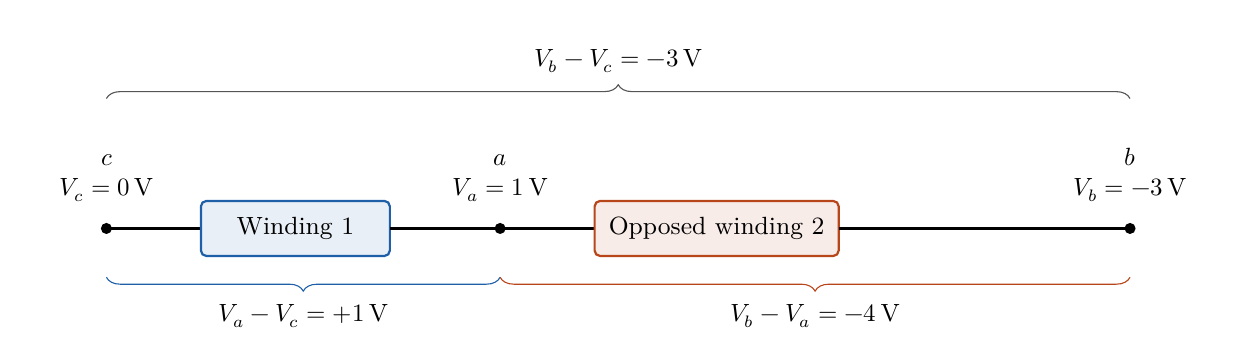
\begin{tikzpicture}
\path[use as bounding box] (0,-1.3) rectangle (15,2.55);
\draw[thick] (1,0)--(2.2,0);
\node[block,massA,minimum width=2.4cm] at (3.4,0) {Winding 1};
\draw[thick] (4.6,0)--(6,0)--(7.2,0);
\node[block,massB,minimum width=3.1cm] at (8.75,0) {Opposed winding 2};
\draw[thick] (10.3,0)--(14,0);
\foreach \x/\n/\v in {1/c/0,6/a/1,14/b/{-3}} {
 \fill (\x,0) circle (2pt);
 \node[above=6pt,align=center] at (\x,0) {$\n$\\$V_\n=\v\,\mathrm{V}$};
}
\draw[decorate,decoration={brace,amplitude=5pt},frameline] (1,1.65)--(14,1.65);
\node[above] at (7.5,1.85) {$V_b-V_c=-3\,\mathrm{V}$};
\draw[decorate,decoration={brace,mirror,amplitude=5pt},elemA] (1,-.62)--(6,-.62);
\node[below] at (3.5,-.84) {$V_a-V_c=+1\,\mathrm{V}$};
\draw[decorate,decoration={brace,mirror,amplitude=5pt},elemB] (6,-.62)--(14,-.62);
\node[below] at (10,-.84) {$V_b-V_a=-4\,\mathrm{V}$};
\end{tikzpicture}
\end{document}
